\documentclass[12pt]{article}

\usepackage[margin=1in]{geometry}
\usepackage{amsmath,amsthm,amssymb,amsfonts}
\usepackage{graphicx}
\usepackage{xcolor}
\usepackage{enumitem}
\usepackage[utf8]{inputenc}
\usepackage{hyperref}
\usepackage{listings}
\usepackage{natbib}

%\lstset{%
%  basicstyle=\footnotesize\ttfamily,
%  keywordstyle=\bfseries\color{green!40!black},
%  commentstyle=\itshape\color{purple!40!black},
%  identifierstyle=\color{blue},
%  stringstyle=\color{orange},
%}

\usepackage[T1]{fontenc}
\usepackage[scaled]{beramono}

\usepackage{color}
\definecolor{bluekeywords}{rgb}{0.13,0.13,1}
\definecolor{greencomments}{rgb}{0,0.5,0}
\definecolor{redstrings}{rgb}{0.9,0,0}

\usepackage{listings}
\lstset{language=Matlab,
showspaces=false,
showtabs=false,
breaklines=true,
showstringspaces=false,
breakatwhitespace=true,
escapeinside={(*@}{@*)},
commentstyle=\color{greencomments},
keywordstyle=\color{bluekeywords}\bfseries,
stringstyle=\color{redstrings},
basicstyle=\ttfamily
}

\author{Jake Snell\\\href{mailto:jsnell@cs.toronto.edu}{\texttt{jsnell@cs.toronto.edu}}}
\title{CSC420: Introduction to Image Understanding\\Assignment 3 Solutions}

\newcommand{\Oh}{\mathcal{O}}

% Wrap all the TA-specific text in this, so we can easily remove it in the
% if we want to distribute the solutions to the student.
\newcommand{\ta}[1]{\textbf{#1}}

\begin{document}

\maketitle

\section*{Problem 1}

The shoe and the bill lie on the same planar surface and so we can use
a homography to transform between a point $\mathbf{p}$ on the image plane and
a point $\mathbf{P}$ in the world plane. Expressing $\mathbf{P}$ and
$\mathbf{p}$ in homogeneous coordinates with homography matrix $\mathbf{H}$, we
have the following:
%
\begin{align}
    \mathbf{P} &= \mathbf{H} \mathbf{p} \\
    \begin{bmatrix} X \\ Y \\ Z \end{bmatrix} &=
        \begin{bmatrix} h_{11} & h_{12} & h_{13} \\
                        h_{21} & h_{22} & h_{23} \\
                        h_{31} & h_{32} & h_{33} \end{bmatrix}
        \begin{bmatrix} x \\ y \\ z \end{bmatrix}
\end{align}
%
We know that a five-dollar bill is $d_1$ = 15.24 cm long and $d_2$ = 6.985 cm
tall\footnote{\texttt{http://www.bankofcanada.ca/banknotes/bank-note-series/polymer/5-polymer-note/}}.
So let's express the bottom-left, bottom-right, top-left, and top-right world
coordinates of the bill, respectively, as follows:
%
\begin{align}
    \mathbf{P}_1 = \begin{bmatrix}0 \\ 0 \\ 1\end{bmatrix},
    \mathbf{P}_2 = \begin{bmatrix}d_1 \\ 0 \\ 1\end{bmatrix},
    \mathbf{P}_3 = \begin{bmatrix}0 \\ d_2 \\ 1\end{bmatrix},
    \mathbf{P}_4 = \begin{bmatrix}d_1 \\ d_2 \\ 1\end{bmatrix}
\end{align}
%
We can extract the corresponding points in the image plane $p_1$, $p_2$, $p_3$,
and $p_4$ directly from the image. Then we can solve for $\mathbf{H}$ using
the technique described in the appendix of \citep{criminisi2002single}. We
solve $\mathbf{A}\mathbf{h} = 0$ for $\|\mathbf{h}\|=1$, where $\mathbf{A}$
and $\mathbf{h}$ are the following:
%
\begin{align}
    \mathbf{A} = \begin{bmatrix}
        x_1 & y_1 & 1 & 0   & 0   & 0 & -x_1 X_1 & -y_1 X_1 & -X_1 \\
        0   & 0   & 0 & x_1 & y_1 & 1 & -x_1 Y_1 & -y_1 Y_1 & -Y_1 \\
        \vdots & \vdots & \vdots & \vdots & \vdots &
        \vdots & \vdots & \vdots & \vdots \\
        x_4 & y_4 & 1 & 0   & 0   & 0 & -x_4 X_4 & -y_4 X_4 & -X_4 \\
        0   & 0   & 0 & x_4 & y_4 & 1 & -x_4 Y_4 & -y_4 Y_4 & -Y_4 \\
    \end{bmatrix} \\
    \mathbf{h} = \begin{bmatrix}
        h_{11} & h_{12} & h_{13} &
        h_{21} & h_{22} & h_{23} &
        h_{31} & h_{32} & h_{33}
    \end{bmatrix}^\top
\end{align}
%
This can be solved by setting $\mathbf{h}$ to be the null vector of
$\mathbf{A}$. With $\mathbf{H}$ now in hand, we can estimate the world
coordinate of any image coordinate by pre-multiplying it by $\mathbf{H}$.
In the end, our estimated shoe length is 27.16 cm and width is 7.86 cm.

% \lstinputlisting[language=Matlab]{prob1.m}

\section*{Problem 2}

\subsection*{Part (a)}

Greedy and RANSAC matchings can be found in Figures~\ref{fig:prob2a_greedy} and
\ref{fig:prob2a_ransac}.

\begin{figure}[ht]
    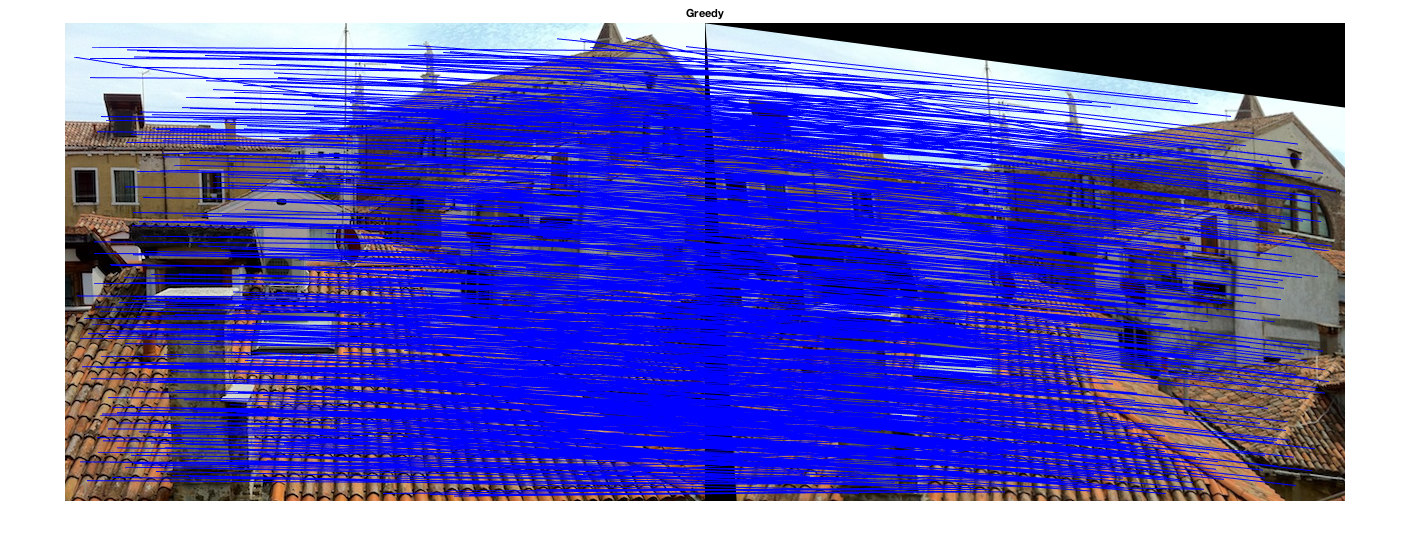
\includegraphics[width=\linewidth]{output/prob2a_output_greedy.png}
    \caption{Greedy Matching}
    \label{fig:prob2a_greedy}
\end{figure}

\begin{figure}[ht]
    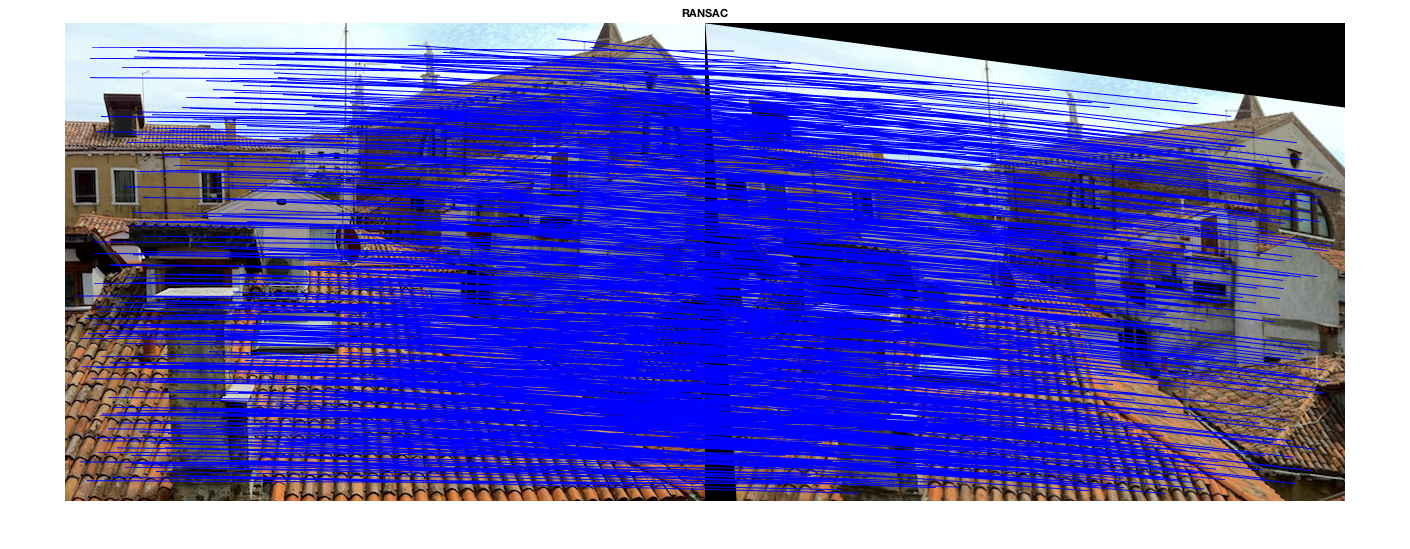
\includegraphics[width=\linewidth]{output/prob2a_output_ransac.png}
    \caption{RANSAC Matching}
    \label{fig:prob2a_ransac}
\end{figure}

\lstinputlisting{output/prob2a_output.txt}

\subsection*{Part (b)}

The reconstructed image can be found in Figure~\ref{fig:prob2b}. The boundaries
are permuted because there are no shared keypoints between the source and target
in the boundaries. Thus they will not enter into either our RANSAC procedure or
the mean residual SSD evaluation.

\begin{figure}[ht]
    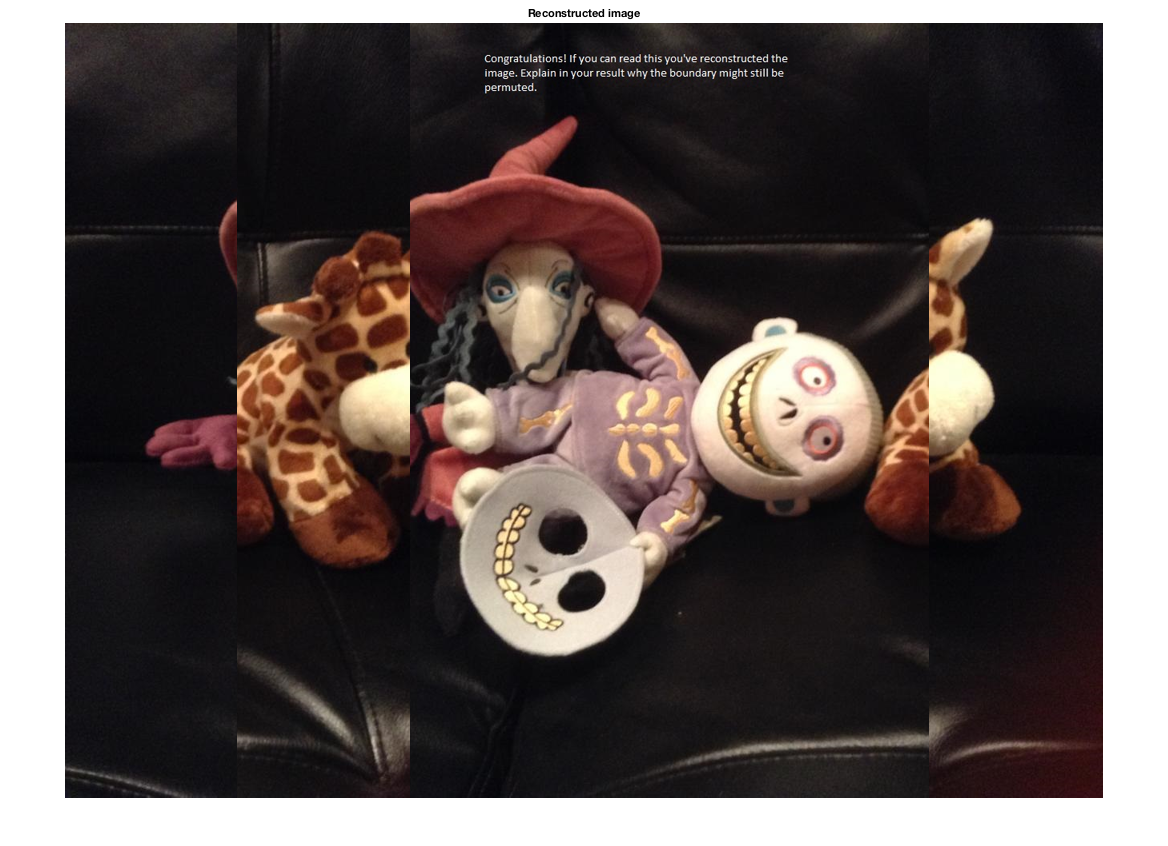
\includegraphics[width=\linewidth]{output/prob2b_output.png}
    \caption{Reconstructed Image}
    \label{fig:prob2b}
\end{figure}

\lstinputlisting{output/prob2b_output.txt}

\section*{Problem 3}

\subsection*{Part (a)}

We will need to collect the image coordinates of three points along a single
rail. Suppose that we have three world points along a rail, each 1 tie apart:
%
\begin{equation}
    V_1 = \begin{bmatrix} X \\ Y \\ Z \\ 1 \end{bmatrix},
    V_2 = \begin{bmatrix} X + D_x \\ Y + D_y \\ Z + D_z \\ 1 \end{bmatrix},
    V_3 = \begin{bmatrix} X + 2 D_x \\ Y + 2 D_y \\ Z + 2 D_z \\ 1 \end{bmatrix}
\end{equation}
%
The corresponding image coordinates $v_1$, $v_2$, and $v_3$ are:
%
\begin{align}
    v_1 = \begin{bmatrix}w_1 x_1 \\ w_1 y_1 \\ w_1 \end{bmatrix} = H V_1,
    v_2 = \begin{bmatrix}w_2 x_2 \\ w_2 y_2 \\ w_2 \end{bmatrix} = H V_2,
    v_3 = \begin{bmatrix}w_3 x_3 \\ w_3 y_3 \\ w_3 \end{bmatrix} = H V_3,
\end{align}
%
where $H = K \begin{bmatrix} \begin{array}{c|c} R  & t \end{array} \end{bmatrix}$.
Subtracting $v_1 = HV_1$ from both $v_2 = Hv_2$ and $v_3 = Hv_3$, we have:
%
\begin{equation}
    \begin{bmatrix} w_2 x_2 - w_1 x_1 \\
        w_2 y_2 - w_1 y_1 \\
        w_2 - w_1 \\
        w_3 x_3 - w_1 x_1 \\
        w_3 y_3 - w_1 y_1 \\
        w_3 - w_1
    \end{bmatrix} = \begin{bmatrix} \, \\ H \\ \, \\ \, \\ H \\ \, \end{bmatrix}
                    \begin{bmatrix} D_x \\ D_y \\ D_z \\ 0 \\ 2D_x \\ 2D_y \\ 2D_z \\ 0 \end{bmatrix},
\end{equation}
%
a linear system of six equations with six unknowns: $w_1, w_2, w_3, D_x, D_y,$
and $D_z$. After solving for $D_x$, $D_y$ and $D_z$, the distance between
adjacent railway ties is $\sqrt{D_x^2 + D_y^2 + D_z^2}$.

\subsection*{Part (b)}

We can use the relationship from Derek Hoiem's notes on single-view
geometry\footnote{\url{https://courses.engr.illinois.edu/cs543/sp2011/materials/3dscene_book_svg.pdf}}.
%
\begin{equation}
    \frac{Y_0}{Y_c} = \frac{v_t - v_b}{v_h - v_b},
    \label{eq:man_geom}
\end{equation}
%
where $Y_0$ is the height of the man, $Y_c$ is the camera height, $v_t$ is
the top of the man in the image, $v_b$ is the bottom of the man in the image,
and $v_h$ is the image height of the horizon. By measuring the image, we find
$v_b = 65$, $v_h = 240$, and $v_t = 359$. Substituting into~\eqref{eq:man_geom},
we can estimate the height of the man to be approximately:
%
\begin{equation}
    Y_0 = Y_c \frac{v_t - v_b}{v_h - v_b} = (95 \text{ cm}) \frac{359 \text{ px} - 65 \text{ px}}
    {240 \text{ px} - 65 \text{ px}} = 159.6 \text{ cm}.
\end{equation}

\section*{Problem 4}

\subsection*{Part (a)}

\begin{equation}
    K = \begin{bmatrix}
        721.5 & 0     & 609.6 \\
        0     & 721.5 & 172.9 \\
        0     & 0     & 1
    \end{bmatrix}
\end{equation}

\subsection*{Part (b)}

\begin{equation}
    Y = -1.7 \text{ m}
\end{equation}

\subsection*{Part (c)}

Since the point is on the ground, $Y = -1.7 \text{ m}$ From similar triangles,
we know:
%
\begin{equation}
    \frac{Z}{1.7 \text{ m}} = \frac{f}{p_y - y} \Rightarrow Z = \left(\frac{721.5}{172.9 - y}\right) (1.7 \text{ m})
\end{equation}
%
Additionally,
%
\begin{equation}
    \frac{X}{Z} = \frac{x - p_x}{f} \Rightarrow X = \left(\frac{x - 609.6}{721.5}\right) Z
\end{equation}
%
Thus the 3D location is:
%
\begin{equation}
    (X, Y, Z) = \left(\left(\frac{x - 609.6}{172.9 - y}\right) (1.7 \text{ m}),
                -1.7 \text{ m}, \left(\frac{721.5}{172.9 - y}\right) (1.7 \text{ m}) \right)
\end{equation}

\section*{Extra Credit}

\subsection*{Part (a)}

Since we are working in the camera coordinate system, we have:
%
\begin{equation}
    \begin{bmatrix}
        w \cdot x \\ w \cdot y \\ w
    \end{bmatrix} =
    \begin{bmatrix}
        fx & 0   & p_x \\
        0  & f_y & p_y \\
        0  & 0   & 1
    \end{bmatrix} \begin{bmatrix} X \\ Y \\ Z \end{bmatrix}
\end{equation}
%
Solving for $X$ and $Y$, we get:
%
\begin{align}
    X &= \frac{Z}{f_x} (x - p_x) \\
    Y &= \frac{Z}{f_y} (y - p_y)
\end{align}
%
The resulting point cloud can be found in Figure~\ref{fig:ec_a}.
%
\begin{figure}
    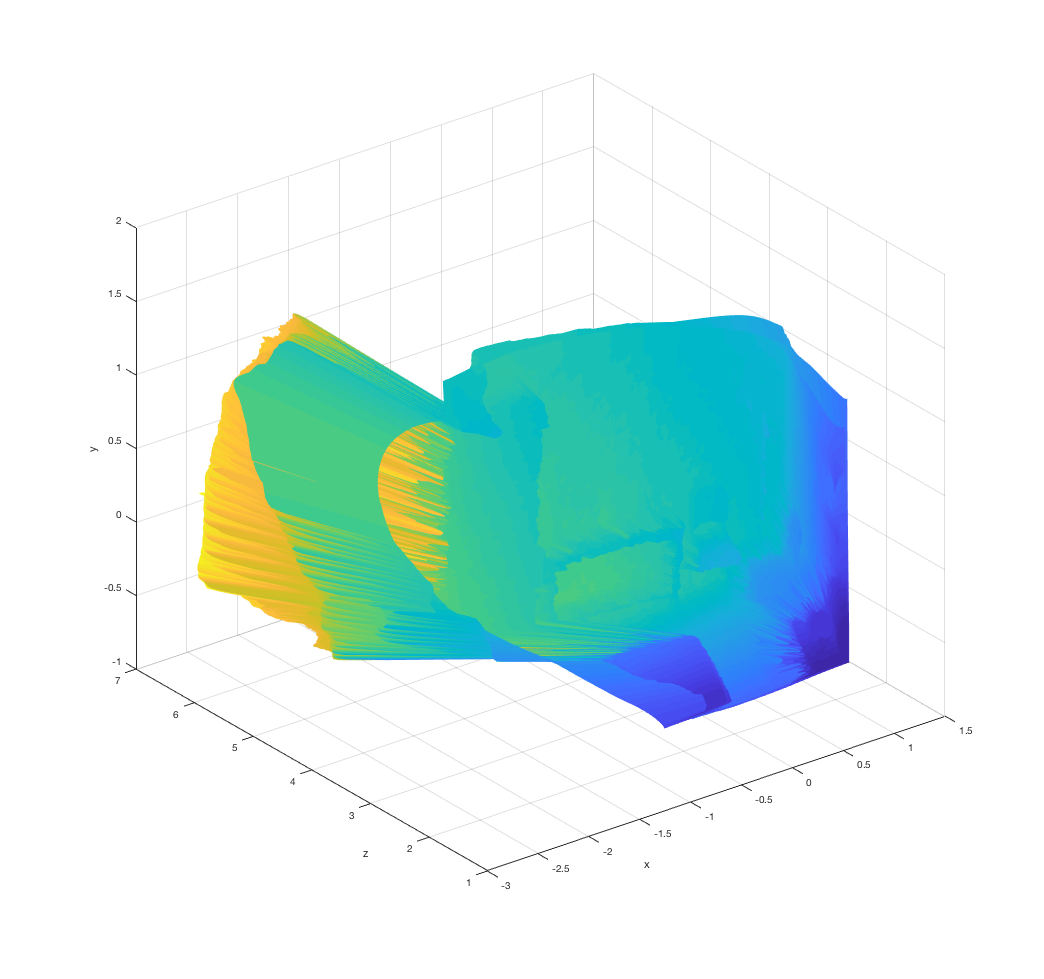
\includegraphics[width=\linewidth]{output/ec_output.png}
    \caption{Point cloud of bedroom image.}
    \label{fig:ec_a}
\end{figure}
%
\subsection*{Part (b)}
%
\lstinputlisting{output/ec_output.txt}

\bibliography{assignment3_solution}
\bibliographystyle{plainnat}

\end{document}
